\documentclass[12pt,a4paper]{article}
\usepackage[utf8]{inputenc}

% Format
\usepackage{layout}

% Font
\usepackage{MinionPro}
\input glyphtounicode
\pdfgentounicode=1
\usepackage{microtype}
\usepackage[super]{nth}
\usepackage{tfrupee}

% Language
\usepackage[british]{babel}

% References
\usepackage[nosectionbib, tocbib, unnumberedbib]{apacite}

% Figures
\usepackage{graphicx}
\usepackage{caption}    
\graphicspath{ {figures/} }

% Tables
\usepackage{booktabs}
\usepackage{tabularx}

% Commands
\newcommand{\pest}[4]{$ \text{Pr} (\text{``us''} | \text{#1}) = #2$, $[#3, #4]$}
\newcommand{\pdif}[4]{$ \Delta\text{Pr} (\text{``us''} | \text{#1}) = #2$, $[#3, #4]$}

\begin{document}

% Captions
\captionsetup[figure]{font={small},labelfont={it},labelformat={default}, labelsep=period}
\captionsetup[table]{font={small},labelfont={it},labelformat={default}, labelsep=period}

\section*{Figures}

\begin{figure}[h]
\centering
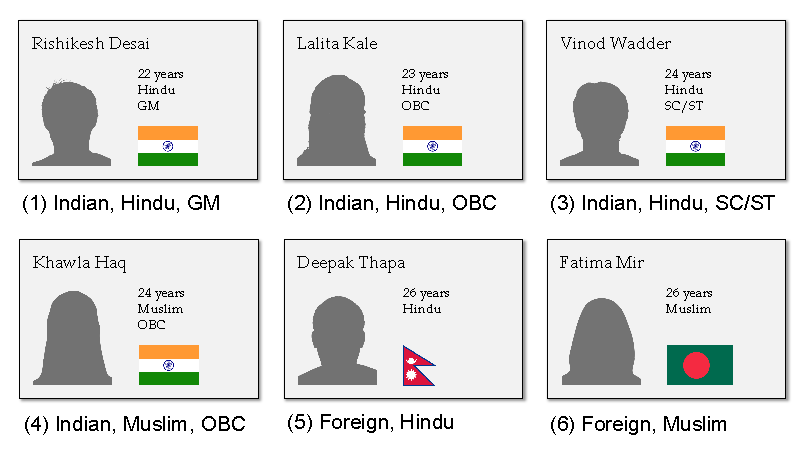
\includegraphics[scale=1]{../figure-1}
\caption{Examples of targets used in the triple crossed-categorization task. \ldots ($N = 26$) \ldots The targets' ages and silhouettes, as well as the order in which they were presented, varied across sessions.}
\label{fig:f1}
\end{figure}

%\begin{figure}[h]
%\centering
%%\includegraphics[scale=1]{../figures/ch4-s4-2}
%\caption{Estimated probability of participants categorizing a target as ``us'' versus ``not us'' by targets' index (\#), nationality, religion, and caste (vertical), and participants' caste membership (horizontal). Dots (•) indicate the most likely \emph{estimate} for a given target's probability of being included in participants' ingroup (in Model~2, Table~\ref{tab:2}), while the shaded ribbons encompass the 67\% (darkest shade), 89\%, and 97\% (lightest shade) most likely estimates of that probability. Pluses (+) indicate the \emph{observed} proportion of participants who included a target in their ingroup.}
%\label{fig:f2}
%\end{figure}

\section*{Tables}

\begin{table}[h]
\caption[Participants by gender, age, nationality, religion, and caste]{Participants by gender, age, nationality, religion, and caste. Categories in \textit{italics} were excluded from the final sample. N/A marks missing responses.}
\centering
\figureversion{lining, tabular}
\small	
\begin{tabular}{llrr} \addlinespace \toprule
\multicolumn{2}{l}{Category} & $n$ & \% \\ \midrule \addlinespace 
Gender      & Woman      & 215 & 61 \\
            & Man & 121 & 34 \\
            & Other & 0 & 0 \\
            & N/A & 15 & 4 \\ \addlinespace \addlinespace
Age         & 18--20 & 1 & 0 \\
            & 21--23 & 254 & 72 \\
            & 24--26 &  77 & 22 \\
            & 27--29 &  10 &  3 \\
            & 30--32 &   1 &  0 \\
            & 33--35 &   0 &  0 \\
            & 36 or older & 1 & 0 \\ 
            & N/A & 7 & 2 \\ \addlinespace \addlinespace
Nationality & Indian & 339 & 97 \\
            & Other & 0 & 0 \\
            & N/A & 12 & 3 \\ \addlinespace \addlinespace
Religion    & Buddhism & 1 & 0 \\ 
            & Christianity & 11 & 3 \\ 
            & Hinduism & 297 & 85 \\ 
            & \textit{Islam} & \textit{27} & \textit{8} \\ 
            & Jainism & 8 & 2 \\ 
            & Other & 2 & 1 \\ 
            & N/A & 5 & 1 \\ \addlinespace \addlinespace
Caste       & General Caste & 104 & 30 \\ 
            & Other Backward Class & 143 & 41 \\ 
            & Scheduled Caste & 54 & 15 \\ 
            & Scheduled Tribe & 23 & 7 \\ 
            & \textit{Other / Not applicable} & \textit{20} & \textit{6} \\ 
            & \textit{N/A} & \textit{7} & \textit{2} \\ \addlinespace \midrule
Total       &   & 351 & 100 \\ \bottomrule
\end{tabular}
\label{tab:ch4-s4-1}
\end{table}

\end{document}